\begin{figure}[ht!]
\centering
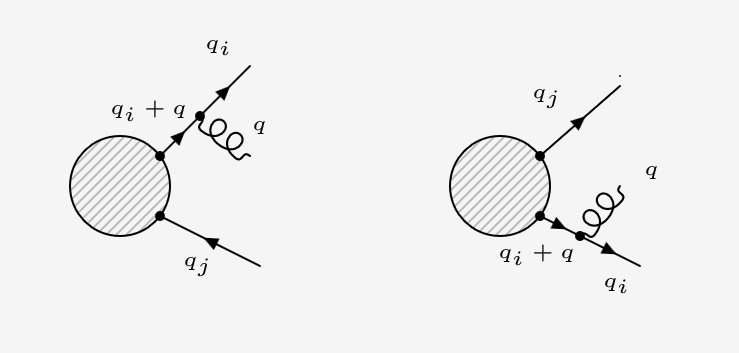
\includegraphics[width=0.85\textwidth]{images/qqg-diagrams.png}
\end{figure}
\pagebreak
\section{qg-$\bar{q}$}

\begin{figure}[h!]
\centering
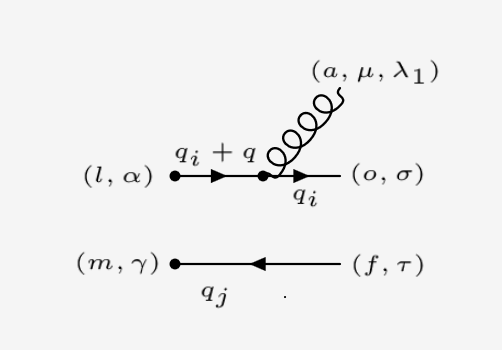
\includegraphics[scale=0.7]{images/qgqbarM.png}
\end{figure}

\begin{equation}
M_1 = [{\bar{u}}_{\sigma}(q_i) (-ig_s \gamma^{\mu}\times {[T^a]_o}^l)  \frac{i(\not{q_i} + \not{q})}{(q_i + q)^2} {\varepsilon^{\lambda_1}}_{\mu} (q)]\: [{v}_{\tau}(q_j)]
\end{equation}

\begin{figure}[h!]
\centering
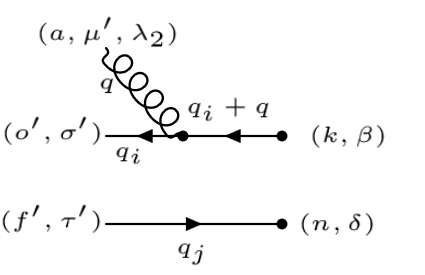
\includegraphics[scale=0.7]{images/qgqbarMDega.png}
\end{figure}

\begin{equation}
{M_1}^{\dagger} = [\frac{-i(\not{q_i} + \not{q})}{(q_i + q)^2} \:  (ig_s \gamma^{{\mu}^{\prime}}\times {[T^b]_{o\:^{\prime}}}^k) \: u_{{\sigma}^{\prime}}(q_i) \: {\varepsilon^{\lambda_2}}_{{\mu}^{\prime}} (q)][{\bar{v}}_{{\tau}^{\prime}}(q_j)]
\end{equation}
\pagebreak
\begin{figure}[h!]
\centering
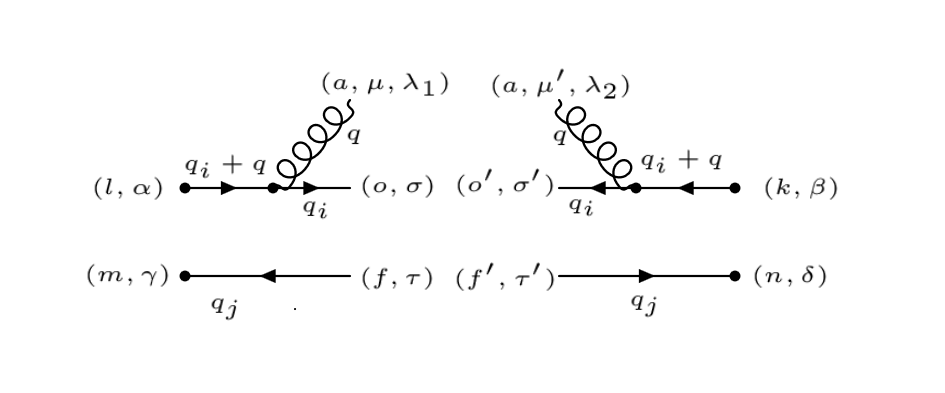
\includegraphics[width=0.85\textwidth]{images/qgqbarMSquer.png}
\end{figure}

\begin{equation}
\begin{split}
|M_1|^2=M_1\:{\color[RGB]{255,0,0} {M_1}^{\dagger}} = [{\bar{u}}_{\sigma}(q_i)\: (-ig_s \gamma^{\mu}\times {[T^a]_o}^l) \: \frac{i(\not{q_i} + \not{q})}{(q_i + q)^2}\:\: {\varepsilon^{\lambda_1}}_{\mu} (q)] [{v}_{\tau}(q_j)]\: \\
\quad\quad\quad\quad\quad\quad\quad\quad\:\:{\color[RGB]{255,0,0}[\frac{-i(\not{q_i} + \not{q})}{(q_i + q)^2} \:  (ig_s \gamma^{{\mu}^{\prime}}\times {[T^b]_{o\:^{\prime}}}^k) \: u_{{\sigma}^{\prime}}(q_i) \: {{\varepsilon^{\lambda_2}}_{{\mu}^{\prime}}}^* (q)][{\bar{v}}_{{\tau}^{\prime}}(q_j)]}
\end{split}
\end{equation}


\begin{equation}
\begin{split}
|M_1|^2=[\frac{-i(\not{q_i} + \not{q})}{(q_i + q)^2} \:
 \:  (ig_s \gamma^{{\mu}^{\prime}}\times {[T^b]_{o\:^{\prime}}}^k) \: {\bar{u}}_{\sigma}(q_i)\:u_{{\sigma}^{\prime}}(q_i) \: {{\varepsilon^{\lambda_2}}_{{\mu}^{\prime}}^* (q) {\varepsilon^{\lambda_1}}_{\mu} (q)} \\
\times (-ig_s \gamma^{\mu}\times {[T^a]_o}^l) \: \frac{i(\not{q_i} + \not{q})}{(q_i + q)^2} ]
[{\bar{v}}_{{\tau}^{\prime}}(q_j) {v}_{\tau}(q_j)]
\end{split}
\end{equation}

and after sum over the lorenz index $({\sigma},{\sigma}^{\prime})$ and $({\tau},{\tau}^{\prime})$ and unsing the spin addition relation:
 
\begin{equation}
\begin{split}
\displaystyle\sum\limits_{{\sigma},{\sigma}^{\prime}} {\bar{u}}_{\sigma}(q_i)\:u_{{\sigma}^{\prime}}(q_i) = \not{q_i} \delta^{{o}{o}^{\prime}},\\
\displaystyle\sum\limits_{{\tau},{\tau}^{\prime}} {\bar{v}}_{\tau}(q_j)\:v_{{\tau}^{\prime}}(q_j) = \not{q_j} \delta^{{f}{f}^{\prime}}
\end{split}
\end{equation}
and sum over polarization index $({\lambda_{1}},{\lambda}_{2})$ :
\begin{equation}
\begin{split}
 \displaystyle\sum\limits_{{\mu},{\mu}^{\prime}} {{\varepsilon^{\lambda_2}}_{{\mu}^{\prime}}^* (q) {\varepsilon^{\lambda_1}}_{\mu} (q)} = -g_{{\mu}{\mu}^{\prime}} \delta^{{a}{b}}
\end{split}
\end{equation}

\begin{equation}
\begin{split}
|M_1|^2=\frac{-g_s^2  {[T^a]_{o}}^k \: {[T^a]_o}^l }{(q_i + q)^2 (q_i + q)^2}
[(\not{q_i} + \not{q}) \:
 \:  \gamma^{{\mu}^{\prime}} \: \not{q_i} \: g_{{{\mu}^{\prime}}{\mu}} 
\gamma^{\mu} \: (\not{q_i} + q)]
[\not{q_j}]
\end{split}
\end{equation}

from here and after contraction between all indices we can actually make statements about the last result.
\begin{equation}
\begin{split}
|M_1|^2=\frac{-g_s^2  {[T^a]_{o}}^k \: {[T^a]_o}^l }{(q_i + q)^2 (q_i + q)^2}
[(\not{q_i} + \not{q}) \:
 \:  \gamma^{{\mu}^{\prime}} \: \not{q_i} \: 
\gamma_{{\mu}^{\prime}} \: (\not{q_i} + q)]
[\not{q_j}]
\end{split}
\end{equation}

In other words we expect the tree level diagram from LO and a number:
\begin{figure}[h!]
\centering
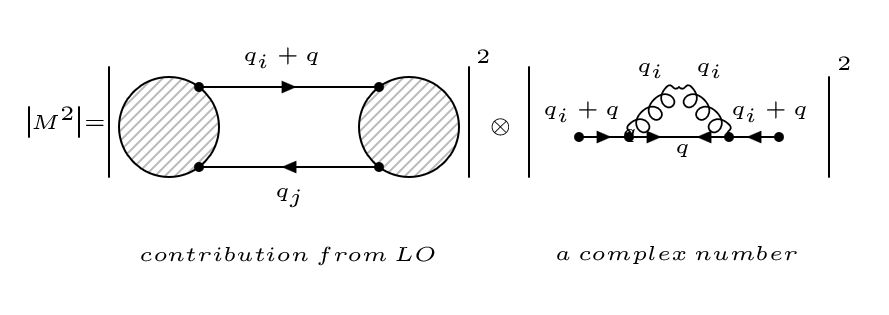
\includegraphics[width=0.85\textwidth]{images/expectationqg-qbar.png}
\end{figure}
Which means:\\
\begin{equation}
\begin{split}
|M_1|^2=\frac{-g_s^2  {[T^a]_{o}}^k \: {[T^a]_o}^l }{(q_i + q)^2 (q_i + q)^2}
[\not{P_i}]
[\not{P_j}]\:\otimes \: {\color[RGB]{255,0,0} (a\: complex\: number)}
\end{split}
\end{equation}  
Let's calculate the contribution and compare the final result with this expectation:
\begin{equation}
\begin{split}
N=: \gamma^{{\mu}^{\prime}} \not{q_i} \: \gamma_{{\mu}^{\prime}} = {q_{i\sigma}} \: \gamma^{{\mu}^{\prime}} \gamma^{\sigma} \:\: \gamma_{{\mu}^{\prime}}\\
={q_{i\sigma}} \: (\lbrace{\gamma^{{\mu}^{\prime}}}, {\gamma^{\sigma}}\rbrace \: - {\gamma^{\sigma}}{\gamma^{{\mu}^{\prime}}})\gamma_{{\mu}^{\prime}}\\
={q_{i\sigma}} \: 2g^{{{\mu}^{\prime}}{\sigma}} \: \gamma_{{\mu}^{\prime}} \: - \:d\:{\gamma^{\sigma}}\\
=(2-d) \not{q_i}
\end{split}
\end{equation}

\begin{equation}
\begin{split}
|M_1|^2=-(2-d)\:\frac{g_s^2  {[T^a]_{o}}^k \: {[T^a]_o}^l }{(q_i + q)^2 (q_i + q)^2}
[(\not{q_i} + \not{q}) \:
 \:\not{q_i} \: 
 \: (\not{q_i} + q)]
[\not{q_j}]
\end{split}
\end{equation}

\begin{equation}
\begin{split}
|M_1|^2=-(2-d)\:\frac{g_s^2  {[T^a]_{o}}^k \: {[T^a]_o}^l }{(q_i + q)^2 (q_i + q)^2}
[\not{q_i} \not{q_i} \not{q_i} \: + \: \not{q_i} \not{q_i} \not{q} \: + \: \not{q} \not{q_i} \not{q_i} \:+\: \not{q} \not{q_i} \not{q}]
[\not{q_j}]
\end{split}
\end{equation}

For the momenta are on-shell which means:
\begin{equation}
\begin{split}
\not{q_i}\not{q_i} = {q_i}^2= {m_i}^2\\
\not{q}\not{q} = {q}^2= {m}^2\\
\not{q_j}\not{q_j} = {q_j}^2= {m_j}^2
\end{split}
\end{equation}

we can first neglect the mass of patrons and ignore each term with $ \not{q_i}\not{q_i} $ and  $ \not{q}\not{q} $ as well.

\begin{equation}
\begin{split}
|M_1|^2=-(2-d)\:\frac{g_s^2  {[T^a]_{o}}^k \: {[T^a]_o}^l }{(2q_i q)(2q_i q)}
[\not{q} \not{q_i} \not{q}]
[\not{q_j}]
\end{split}
\end{equation}

\begin{equation}
\begin{split}
L=\not{q} \not{q_i} \not{q} =\not{q}[{q_{i\sigma}} q_{\mu} \: (\lbrace{\gamma^{\mu}}, {\gamma^{\sigma}}\rbrace - {\gamma^{\sigma}}{\gamma^{\mu}})]\\ 
\not{q}[2{q_{i}}^{\mu} q_{\mu} - {q_{i\sigma}}q_{\mu}{\gamma^{\mu}}{\gamma^{\sigma}}\\
=\not{q} (2q_i q)-q_{\mu}{q_{i\sigma}}q_{\mu}[{\gamma^{\mu}}{\gamma^{\mu}}{\gamma^{\sigma}}]\\
=\not{q} (2q_i q)-q_{\mu}{q_{i\sigma}}q_{\mu}[\frac{{\gamma^{\mu}}{\gamma^{\mu}}}{2} +\frac{{\gamma^{\mu}}{\gamma^{\mu}}}{2}]{\gamma^{\sigma}}\\
=\not{q} (2q_i q)-q_{\mu}{q_{i\sigma}}q_{\mu}[g^{{\mu}{\mu}}]{\gamma^{\sigma}}\\
=\not{q} (2q_i q)-q_{\mu}{q_{i\sigma}}q^{\mu}{\gamma^{\sigma}}\\
=\not{q} (2q_i q)-q^2 \not{q_i}\\
=\not{q} (2q_i q)
\end{split}
\end{equation}
After inserting the last result of $ L $ and simplify the term $ (2q_i q) $ from the denominator and nominator because , we get:
\begin{equation}
\begin{split}
|M_1|^2=-(2-d)\:\frac{g_s^2  {[T^a]_{o}}^k \: {[T^a]_o}^l }{2y(1-2z+2z^2)(p_i \cdot p_j)}
[\not{q}]
[\not{q_j}]
\end{split}
\end{equation}
Now we are going to use the parametrisation from equation (1) to reduce the 3-member matrix element to 2-member and take out the singularity term from the amplitude.
\begin{equation}
\begin{split}
|M_1|^2=(d-2)\:\frac{g_s^2  {[T^a]_{o}}^k \: {[T^a]_o}^l }{2y(1-2z+2z^2)(p_i \cdot p_j)}
[(1-z) \not{p_i}+zy \not{p_j} - \sqrt{zy(1-z)} \not{{m}_{\bot}}]
[(1-y) \not{p_j}]
\end{split}
\end{equation}
Multiplying the both sides 
\begin{equation}
\begin{split}
|M_1|^2=(d-2)\:\frac{g_s^2  {[T^a]_{o}}^k \: {[T^a]_o}^l }{2y(1-2z+2z^2)(p_i \cdot p_j)}
[(1-z)(1-y) \not{p_i}\not{p_j} \\
+zy(1-y) \not{p_j}\not{p_j} + (1-y)\sqrt{zy(1-z)} \not{{m}_{\bot}}\not{p_j}]
\end{split}
\end{equation}
and under consideration of the fact that $ p_i $ and $ p_j $ are the on-shell momenta of the emitter and spectator partons, we can ignore the terms with $ \not{p_i} \not{p_i} $ and $ \not{p_j} \not{p_j} $.
The $ {p_i} \cdot  {m}_{\bot} $ and $ {p_j} \cdot  {m}_{\bot} $ are always $ 0 $ because the $ p_i $ and $ p_j $ are lightlike, i.e. zero transverse component. So those terms can be neglected.


\begin{equation}
\begin{split}
|M_1|^2=(d-2)(1-z)(1-y)\:\frac{g_s^2  {[T^a]_{o}}^k \: {[T^a]_o}^l }{2y(1-2z+2z^2)(p_i \cdot p_j)}
[\not{p_i}][\not{p_j}]
\end{split}
\end{equation}
\pagebreak
\subsection*{with the new parametrisation}

\begin{equation}
\begin{split}
|M_1|^2=(d-2)\:\frac{g_s^2  C_F }{(2k_1\cdot q_i)}
[\not{k_1} ][\not{q_k}]
\end{split}
\end{equation}

\begin{equation}
\begin{split}
&|M_1|^2=(d-2)\:\frac{g_s^2 \: C_F }{2y\: p_i \cdot Q}
[(\alpha_1 -y\beta_1(\frac{Q^2}{2p_i \cdot Q})) \not{p_i} + y\beta_1\not{Q} + \sqrt{y\alpha_1\beta_1}\not{n}_{\bot,1} ]\\
&[A_1\not{p_i} + A_2\not{Q} + \sqrt{1-y}\not{p_k}]
\end{split}
\end{equation}

\begin{equation}
\begin{split}
&|M_1|^2=(d-2)\:\frac{g_s^2 \: C_F }{2y\: p_i \cdot Q}
[(A_2(\alpha_1 -y\beta_1(\frac{Q^2}{2p_i \cdot Q}))+ A_1y\beta_1) {p_i}\cdot Q\\
&+(\alpha_1 -y\beta_1(\frac{Q^2}{2p_i \cdot Q}))\sqrt{1-y}p_i\cdot p_k+A_2 y\beta_1 Q^2+ \sqrt{1-y}\sqrt{y\alpha_1\beta_1}{n}_{\bot,1}\cdot p_k ]\\
\end{split}
\end{equation}

For the collinearity $ y \rightarrow 0 $ we'll get:

\begin{equation}
\begin{split}
&|M_1|^2=(d-2)\:\frac{g_s^2 \: C_F }{2y\: p_i \cdot Q}
[(A_2(\alpha_1 -y\beta_1(\frac{Q^2}{2p_i \cdot Q}))+ A_1y\beta_1) \not{p_i} \not{Q}\\
&+(\alpha_1 -y\beta_1(\frac{Q^2}{2p_i \cdot Q}))\sqrt{1-y}\not{p_i} \not{p_k}+A_2 y\beta_1 Q^2+ \sqrt{1-y}\sqrt{y\alpha_1\beta_1}\not{n}_{\bot,1} \not{p_k} ]\\
\end{split}
\end{equation}

\begin{equation}
\begin{split}
&|M_1|^2=(d-2)(1-\beta_1)\sqrt{1-y}\:\frac{g_s^2 \: C_F }{2y\: p_i \cdot Q}
[\not{p_i} \not{p_k} ]\\
\end{split}
\end{equation}


\newpage

\section{$\bar{q}$g-q}

\begin{figure}[h!]
\centering
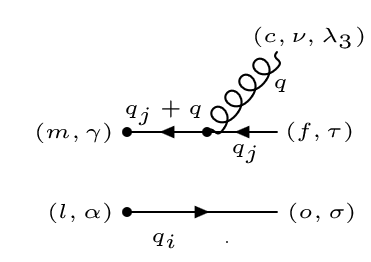
\includegraphics[scale=0.7]{images/qbargqM.png}
\end{figure}

\begin{equation}
M_2 = [\frac{i(\not{q_j} + \not{q})}{(q_j + q)^2} (-ig_s \gamma^{\nu}\times {[T^c]_f}^m) \:{v}_{\tau}(q_j)\: {\varepsilon^{\lambda_3}}_{\nu} (q)]\: [{u}_{\sigma}(q_i)]
\end{equation}
\begin{figure}[h!]
\centering
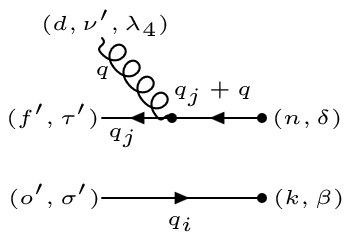
\includegraphics[scale=0.7]{images/qbargqMDega.png}
\end{figure}
\begin{equation}
M_2^{\dagger} = [\bar{v}_{{\tau}^{\prime}}(q_j) \: (ig_s \gamma^{{\nu}^{\prime}}\times {[T^d]_{f^{\prime}}}^n) \: \frac{-i(\not{q_j} + \not{q})}{(q_j + q)^2} \: {\varepsilon^{\lambda_4}}_{{\nu}^{\prime}} (q)]\: [\bar{u}_{{\sigma}^{\prime}}(q_i)]
\end{equation}

\begin{figure}[h!]
\centering
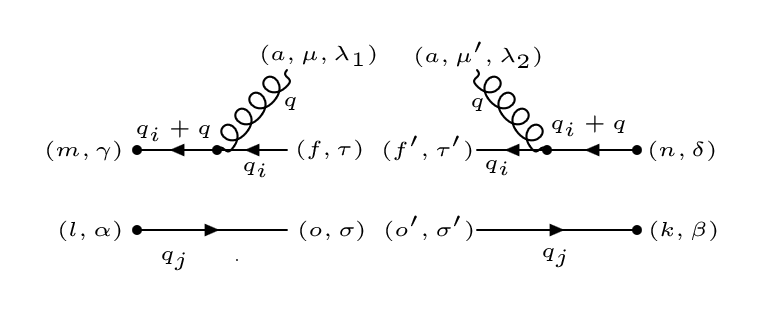
\includegraphics[width=0.85\textwidth]{images/qbargqMSquer.png}
\end{figure}

\begin{equation}
\begin{split}
|M_2|^2=M_2\:{\color[RGB]{255,0,0} {M_2}^{\dagger}} = [\frac{i(\not{q_j} + \not{q})}{(q_j + q)^2} (-ig_s \gamma^{\nu}\times {[T^c]_f}^m) \:{v}_{\tau}(q_j)\: {\varepsilon^{\lambda_3}}_{\nu} (q)]\: [{u}_{\sigma}(q_i)]\: \\
\quad\quad\quad\quad\quad\quad\quad\quad\:\:{\color[RGB]{255,0,0}[\bar{v}_{{\tau}^{\prime}}(q_j) \: (ig_s \gamma^{{\nu}^{\prime}}\times {[T^d]_{f^{\prime}}}^n) \: \frac{-i(\not{q_j} + \not{q})}{(q_j + q)^2} \: {\varepsilon^{\lambda_4}}_{{\nu}^{\prime}} (q)]\: [\bar{u}_{{\sigma}^{\prime}}(q_i)]}
\end{split}
\end{equation}


\begin{equation}
\begin{split}
|M_2|^2 =\frac{g_s^2 \: {[T^c]_f}^m \: {[T^d]_{f^{\prime}}}^n }{(q_j + q)^2 (q_j + q)^2} [(\not{q_j} + \not{q}) \gamma^{\nu}  \:{v}_{\tau}(q_j)\bar{v}_{{\tau}^{\prime}}(q_j)\: {\varepsilon^{\lambda_3}}_{\nu} (q){\varepsilon^{\lambda_4}}_{{\nu}^{\prime}}  (q) \gamma^{{\nu}^{\prime}}(\not{q_j} + \not{q})]\: \\
[{u}_{\sigma}(q_i) ]
\: [\bar{u}_{{\sigma}^{\prime}}(q_i)]
\end{split}
\end{equation}

and after sum over the lorenz index $({\sigma},{\sigma}^{\prime})$ and $({\tau},{\tau}^{\prime})$ and unsing the spin addition relation:
 
\begin{equation}
\begin{split}
\displaystyle\sum\limits_{{\sigma},{\sigma}^{\prime}} {\bar{u}}_{\sigma}(q_i)\:u_{{\sigma}^{\prime}}(q_i) = \not{q_i} \delta^{{o}{o}^{\prime}},\\
\displaystyle\sum\limits_{{\tau},{\tau}^{\prime}} {\bar{v}}_{\tau}(q_j)\:v_{{\tau}^{\prime}}(q_j) = \not{q_j} \delta^{{f}{f}^{\prime}}
\end{split}
\end{equation}
and sum over polarization index $({\lambda_{3}},{\lambda}_{4})$ :
\begin{equation}
\begin{split}
 \displaystyle\sum\limits_{{\nu},{\nu}^{\prime}} {{\varepsilon^{\lambda_4}}_{{\nu}^{\prime}}^* (q) {\varepsilon^{\lambda_3}}_{\nu} (q)} = -g_{{\nu}{\nu}^{\prime}} \delta^{{c}{d}}
\end{split}
\end{equation}

\begin{equation}
\begin{split}
|M_2|^2 =\frac{g_s^2 \: {[T^c]_f}^m \: {[T^c]_{f}}^n }{(q_j + q)^2 (q_j + q)^2} [(\not{q_j} + \not{q}) \gamma^{\nu}  \:\not{q_j}\: (-g_{{\nu}{{\nu}^{\prime}}}) \gamma^{{\nu}^{\prime}}(\not{q_j} + \not{q})]\: 
[\not{q_i} ]
\end{split}
\end{equation}

After the same calculation from the last part, we'll get:

\begin{equation}
\begin{split}
|M_2|^2 =(d-2) \frac{g_s^2 \: {[T^c]_f}^m \: {[T^c]_{f}}^n }{(2qq_j)} [\not{q}]\: 
[\not{q_i} ]
\end{split}
\end{equation}
finally:
\begin{equation}
\begin{split}
|M_2|^2=-(d-2)yz^2\:\frac{g_s^2 \: {[T^c]_f}^m \: {[T^c]_{f}}^n }{2(1-z)(1-y)(p_i \cdot p_j)}
[\not{p_i}][\not{p_j}]
\end{split}
\end{equation}
\newpage

\subsection*{with the new kinematic}

\begin{equation}
\begin{split}
|M_2|^2 =(d-2) \frac{g_s^2 \: {[T^c]_f}^m \: {[T^c]_{f}}^n }{2k_1 \cdot q_k} [\not{k_1}]\: 
[\not{q_i} ]
\end{split}
\end{equation}

\begin{equation}
\begin{split}
&|M_2|^2 =(d-2) \frac{g_s^2 \: C_F}{2k_1 \cdot q_k} [(\alpha_1 -y\beta_1(\frac{Q^2}{2p_i \cdot Q})) \not{p_i} + y\beta_1\not{Q} + \sqrt{y\alpha_1\beta_1}\not{n}_{\bot,1}]\: \\
&[(\beta_1 -\alpha_1 y(\frac{Q^2}{2p_i \cdot Q}))\not{p_i} + y\alpha_1\not{Q} - \sqrt{y\alpha_1\beta_1}\not{n}_{\bot,l} ]
\end{split}
\end{equation}


\begin{equation}
\begin{split}
&|M_2|^2 =(d-2) \frac{g_s^2 \: C_F}{2k_1 \cdot q_k} [y\alpha_1(\alpha_1 -y\beta_1(\frac{Q^2}{2p_i \cdot Q}))\not{p_i}\not{Q}  + y\beta_1(\beta_1 -\alpha_1 y(\frac{Q^2}{2p_i \cdot Q}))]\not{Q}\not{p_i}\\
&+y^2\alpha_1\beta_1 Q^2-y\beta_1\sqrt{y\alpha_1\beta_1}\not{Q}\not{n}_{\bot,1}+y\beta_1\sqrt{y\alpha_1\beta_1}\not{n}_{\bot,1}\not{Q}- y\alpha_1\beta_1 \:{{n}_{\bot,l}}^2 \\
&+ (\beta_1 -\alpha_1 y(\frac{Q^2}{2p_i \cdot Q})\sqrt{y\alpha_1\beta_1}\not{n}_{\bot,1}\not{p_i}- (\alpha_1 -\alpha_1 y(\frac{Q^2}{2p_i \cdot Q})\sqrt{y\alpha_1\beta_1}\not{p_i}\not{n}_{\bot,1} ]
\end{split}
\end{equation}

Which means:
\begin{equation}
\begin{split}
&|M_2|^2 \sim(d-2) \frac{g_s^2 \: C_F}{2k_1 \cdot q_k} y[...]\\
&\:\:\:\:\:\:\:\:|M_2|^2\rightarrow 0 \:\:\:\:\:\:\:\text{for}\:\:\:\:\: y\rightarrow 0
\end{split}
\end{equation}
\newpage

\section{$M_1 {M_2}^{\dagger}$}

\begin{figure}[h!]
\centering
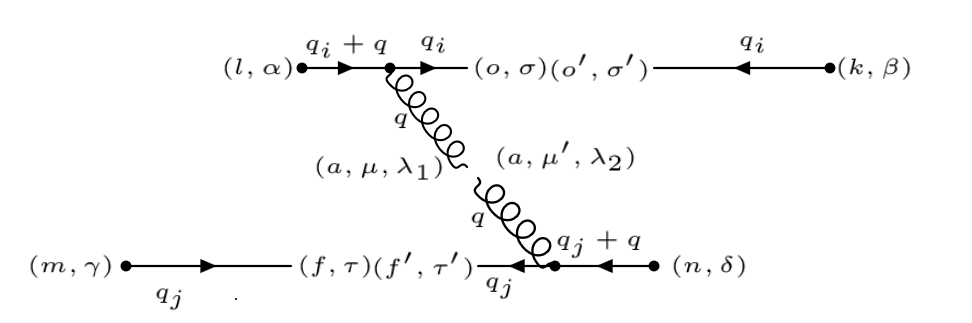
\includegraphics[width=0.85\textwidth]{images/M1M2Degaqqg.png}
\end{figure}

\begin{equation}
\begin{split}
M_1\:{\color[RGB]{255,0,0} {M_2}^{\dagger}} = [{\bar{u}}_{\sigma}(q_i)\: (-ig_s \gamma^{\mu}\times {[T^a]_o}^l) \: \frac{i(\not{q_i} + \not{q})}{(q_i + q)^2}\:\: {\varepsilon^{\lambda_1}}_{\mu} (q)] [{v}_{\tau}(q_j)]\: \\
\quad\quad\quad\quad\quad\quad\quad\quad\:\:{\color[RGB]{255,0,0}[\bar{v}_{{\tau}^{\prime}}(q_j) \: (ig_s \gamma^{{\nu}^{\prime}}\times {[T^d]_{f^{\prime}}}^n) \: \frac{-i(\not{q_j} + \not{q})}{(q_j + q)^2} \: {\varepsilon^{\lambda_4}}_{{\nu}^{\prime}} (q)]\: [{u}_{{\sigma}^{\prime}}(q_i)]}
\end{split}
\end{equation}



\begin{equation}
\begin{split}
M_1\: {M_2}^{\dagger} = \frac{g_s^2 {[T^a]_o}^l \:{[T^d]_{f^{\prime}}}^n }{(2q_i q)(2q_j q)} [\not{q_i}\: \gamma^{\mu} \: (\not{q_i} + \not{q})\: ]{\varepsilon^{\lambda_1}}_{\mu} (q) \: {\varepsilon^{\lambda_4}}_{{\nu}^{\prime}} (q) \\
\:[\not{q_j} \:\gamma^{{\nu}^{\prime}} \: (\not{q_j} + \not{q})]\:
\end{split}
\end{equation}

\begin{equation}
\begin{split}
M_1\: {M_2}^{\dagger} = \frac{g_s^2 {[T^a]_o}^l \:{[T^a]_{f^{\prime}}}^n }{(2q_i q)(2q_j q)} [\not{q_i}\: \gamma^{\mu} \: (\not{q_i} + \not{q})\: ] -g_{{\mu}{{\nu}^{\prime}}} \\
\:[\not{q_j} \:\gamma^{{\nu}^{\prime}} \: (\not{q_j} + \not{q})]\:
\end{split}
\end{equation}



\begin{equation}
\begin{split}
M_1\: {M_2}^{\dagger} = \frac{-g_s^2 {[T^a]_o}^l \:{[T^a]_{f^{\prime}}}^n }{(2q_i q)(2q_j q)} [\not{q_i}\: \gamma^{\mu} \: (\not{q_i} + \not{q})\: ]
\:[\not{q_j} \:\gamma_{\mu} \: (\not{q_j} + \not{q})]\:
\end{split}
\end{equation}

Expectation:
\begin{figure}[h!]
\centering
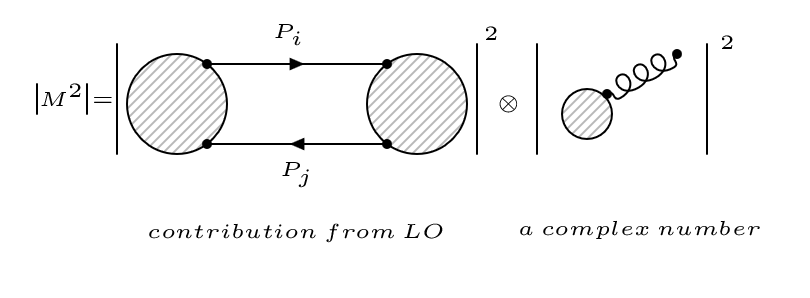
\includegraphics[width=0.85\textwidth]{images/expectationM1M2dagger.png}
\end{figure}


\begin{equation}
\begin{split}
M_1\: {M_2}^{\dagger} = \frac{-g_s^2 {[T^a]_o}^l \:{[T^a]_{f^{\prime}}}^n }{(2q_i q)(2q_j q)} [(\not{q_i} + \not{q})\: \gamma^{\mu} \:  \not{q_i}\:]
\:[(\not{q_j} + \not{q}) \:\gamma_{\mu} \:\not{q_j} ]\:
\end{split}
\end{equation}


\begin{equation}
\begin{split}
M_1\: {M_2}^{\dagger} = \frac{-g_s^2 {[T^a]_o}^l \:{[T^a]_{f^{\prime}}}^n }{(2q_i q)(2q_j q)} [-(\not{q_i} + \not{q})\:\not{q_i}\: \gamma^{\mu} \:+2(\not{q_i} + \not{q})\:{q_{i}}^{\mu}]\\
\:[-(\not{q_j} + \not{q}) \not{q_j} \:\gamma_{\mu} \: + 2(\not{q_j} + \not{q}) {q_{j{\mu}}}]\:
\end{split}
\end{equation}


\begin{equation}
\begin{split}
&M_1\: {M_2}^{\dagger} = \frac{-g_s^2 {[T^a]_o}^l \:{[T^a]_{f^{\prime}}}^n }{(2q_i q)(2q_j q)} 
[(\not{q_i} + \not{q})\:\not{q_i}\: \gamma^{\mu}] \:[(\not{q_j} + \not{q}) \not{q_j} \gamma_{\mu}] \\
&-2[(\not{q_i} + \not{q})\:\not{q_i}\: \gamma^{\mu}]\:[ (\not{q_j} + \not{q}) {q_{j{\mu}}}]
\:-2[(\not{q_i} + \not{q})\:{q_{i}}^{\mu}][(\not{q_j} + \not{q}) \not{q_j} \:\gamma_{\mu}]\\
&+4[(\not{q_i} + \not{q})\:{q_{i}}^{\mu}][(\not{q_j} + \not{q}) {q_{j{\mu}}}]
\end{split}
\end{equation}

\begin{equation}
\begin{split}
&M_1\: {M_2}^{\dagger} = \frac{-g_s^2 {[T^a]_o}^l \:{[T^a]_{f^{\prime}}}^n }{(2q_i q)(2q_j q)} 
[(\not{q_i} + \not{q})\:\not{q_i}\: \gamma^{\mu}] \:[(\not{q_j} + \not{q}) \not{q_j} \gamma_{\mu}] \\
&-2[(\not{q_i} + \not{q})\:\not{q_i}\:\not{q_{j}} ]\:[ \not{q_j} + \not{q} ]
\:-2[\not{q_i} + \not{q}\:][(\not{q_j} + \not{q}) \not{q_j} \:\not{q_i}]\\
&+4[(\not{q_i} + \not{q})\:{q_{i}}^{\mu}][(\not{q_j} + \not{q}) {q_{j{\mu}}}]
\end{split}
\end{equation}

\begin{equation}
\begin{split}
&M_1\: {M_2}^{\dagger} = \frac{-g_s^2 {[T^a]_o}^l \:{[T^a]_{f^{\prime}}}^n }{(2q_i q)(2q_j q)} 
[(\not{q_i} + \not{q})\:\not{q_i}\: \gamma^{\mu}] \:[(\not{q_j} + \not{q}) \not{q_j} \gamma_{\mu}] \\
&+4[(\not{q_i} + \not{q})\:{q_{i}}^{\mu}][(\not{q_j} + \not{q}) {q_{j{\mu}}}]
\end{split}
\end{equation}

\begin{equation}
\begin{split}
M_1\: {M_2}^{\dagger} = \frac{-g_s^2 \:\:{[T^a]_o}^l \:{[T^a]_{f^{\prime}}}^n }{4(1-z)(1-y)y(1-2z+2z^2)(p_i \cdot p_j)(p_i \cdot p_j)} \\
[y(1-2z+2z^2)\not{p_i}\:\not{p_j}\: \gamma^{\mu}] \:[(1-z)(1-y)\not{p_i} \not{p_j} \gamma_{\mu}] \\
+4({q_{i}}^{\mu} \cdot {q_{j{\mu}}})[(\not{q_i} + \not{q})][(\not{q_j} + \not{q})]
\end{split}
\end{equation}

\begin{equation}
\begin{split}
M_1\: {M_2}^{\dagger} = \frac{-g_s^2 \:\:{[T^a]_o}^l \:{[T^a]_{f^{\prime}}}^n }{4(1-z)(1-y)y(1-2z+2z^2)(p_i \cdot p_j)(p_i \cdot p_j)} \\
[y(1-2z+2z^2)\not{p_i}\:\not{p_j}\: \gamma^{\mu}] \:[(1-z)(1-y)\not{p_i} \not{p_j} \gamma_{\mu}] \\
+4(p_i \cdot p_j)[(\not{p_i} + y\not{p_j})][(1-z)\not{p_i} + (1+yz-y) \not{p_j} - \sqrt{zy(1-z)}\not{m}]
\end{split}
\end{equation}

\begin{equation}
\begin{split}
M_1\: {M_2}^{\dagger} = \frac{-g_s^2 \:\:{[T^a]_o}^l \:{[T^a]_{f^{\prime}}}^n }{(1-z)(1-y)y(1-2z+2z^2)(p_i \cdot p_j)} 
z(1-y)[\not{p_i}][\not{p_j}]
\end{split}
\end{equation}







\begin{equation}
\begin{split}
M_1\: {M_2}^{\dagger} = \frac{-g_s^2 \:\:{[T^a]_o}^l \:{[T^a]_{f^{\prime}}}^n }{(1-z)y(1-2z+2z^2)(p_i \cdot p_j)} 
z[\not{p_i}][\not{p_j}]
\end{split}
\end{equation}

\pagebreak

\subsection*{With the new kinematic}

\begin{equation}
\begin{split}
&M_1\: {M_2}^{\dagger} = \frac{-g_s^2 {[T^a]_o}^l \:{[T^a]_{f^{\prime}}}^n }{(2q_i k_1)(2q_k k_1)} 
[(\not{q_i} + \not{k_1})\:\not{q_i}\: \gamma^{\mu}] \:[(\not{q_k} + \not{k_1}) \not{q_k} \gamma_{\mu}] \\
&+4[(\not{q_i} + \not{k_1})\:{q_{i}}^{\mu}][(\not{q_k} + \not{k_1}) {q_{k{\mu}}}]
\end{split}
\end{equation}

\begin{equation}
\begin{split}
&M_1\: {M_2}^{\dagger} = \frac{-g_s^2\: C_F }{4y(1-\beta_1) (1-y)\:(p_i \cdot p_k)(p_i \cdot Q)} \\
&[(\not{q_i}\not{q_i} + \not{k_1}\not{q_i})\: \gamma^{\mu}] [(\not{q_k}\not{q_k} + \not{k_1}\not{q_k})  \gamma_{\mu}] +4({{q_{i}}^{\mu}q_{k{\mu}}})[\not{q_i} + \not{k_1}\:][\not{q_k} + \not{k_1} ]
\end{split}
\end{equation}

\begin{equation}
\begin{split}
&M_1\: {M_2}^{\dagger} = \frac{-g_s^2\: C_F }{4y(1-\beta_1) (1-y)\:(p_i \cdot p_k)(p_i \cdot Q)} \\
&[\not{k_1}\not{q_i}\: \gamma^{\mu}] [ \not{k_1}\not{q_k}  \gamma_{\mu}] +4({q_{i}}\cdot q_k)[\not{q_i}\not{q_k} + \not{k_1}\not{q_k}+\not{q_i}\not{k_1} ]
\end{split}
\end{equation}

\begin{equation}
\begin{split}
&M_1\: {M_2}^{\dagger} = \frac{-g_s^2\: C_F }{4y(1-\beta_1) (1-y)\:(p_i \cdot p_k)(p_i \cdot Q)} \\
&4(A_1\beta_1 {p_i}\cdot{p_i}+A_2\beta_1 {p_i}\cdot {{Q}}+\beta_1 \sqrt{1-y}{p_i}\cdot {{p_k}})\\
&[A_1\beta_1 \not{p_i}\not{p_i}+A_2\beta_1 \not{p_i}\not{Q}+\beta_1 \sqrt{1-y}\not{p_i} \not{p_k}\\
&+ [(1-\beta_1)-y\beta_1 (\frac{Q^2}{2p_i \cdot Q})] \sqrt{1-y}\not{p_i}\not{p_k}-y {\beta_1} (\frac{Q^2}{2p_i \cdot Q}) A_1 \:\not{p_i}\not{p_i}\\
&-y {\beta_1} (\frac{Q^2}{2p_i \cdot Q}) A_2\: \not{p_i}\not{Q}+y {\beta_1} A_1 \:\not{Q}\not{p_i}+y {\beta_1} A_2 \:\not{Q}\not{Q}+y {\beta_1}\sqrt{1-y}\not{Q}\not{p_k}\\
&+[\beta_1(1-\beta_1)-y {\beta_1}^2 (\frac{Q^2}{2p_i \cdot Q})] \not{p_i}\not{p_i}+y {\beta_1}^2 \not{p_i}\not{Q} ]
\end{split}
\end{equation}

\begin{equation}
\begin{split}
&M_1\: {M_2}^{\dagger} = \frac{-g_s^2\: C_F }{4y(1-\beta_1) (1-y)\:(p_i \cdot p_k)(p_i \cdot Q)} \\
&4(A_2\beta_1 {p_i}\cdot {{Q}}+\beta_1 \sqrt{1-y}{p_i}\cdot {{p_k}})[A_2\beta_1 \not{p_i}\not{Q}+\beta_1 \sqrt{1-y}\not{p_i} \not{p_k}\\
&+ [(1-\beta_1)-y\beta_1 (\frac{Q^2}{2p_i \cdot Q})] \sqrt{1-y}\not{p_i}\not{p_k}-y {\beta_1} (\frac{Q^2}{2p_i \cdot Q}) A_2\: \not{p_i}\not{Q}\\
&+y {\beta_1} A_1 \:\not{Q}\not{p_i}+y {\beta_1} A_2 \:\not{Q}\not{Q}+y {\beta_1}\sqrt{1-y}\not{Q}\not{p_k}+y {\beta_1}^2 \not{p_i}\not{Q} ]
\end{split}
\end{equation}

\begin{equation}
\begin{split}
&M_1\: {M_2}^{\dagger} = \frac{-g_s^2\: C_F }{4y(1-\beta_1) (1-y)\:(p_i \cdot p_k)(p_i \cdot Q)} \\
&4(\beta_1 \sqrt{1-y}{p_i}\cdot {{p_k}})[\beta_1 \sqrt{1-y}\not{p_i} \not{p_k}+ (1-\beta_1) \sqrt{1-y}\not{p_i}\not{p_k}]
\end{split}
\end{equation}

\begin{equation}
\begin{split}
&M_1\: {M_2}^{\dagger} = \frac{-g_s^2\: C_F }{y(1-\beta_1) \:(p_i \cdot p_k)(p_i \cdot Q)} \beta_1( {p_i}\cdot {{p_k}})[\beta_1 \not{p_i} \not{p_k}+ (1-\beta_1) \not{p_i}\not{p_k}]
\end{split}
\end{equation}

\begin{equation}
\begin{split}
&M_1\: {M_2}^{\dagger} = \frac{\beta_1}{(1-\beta_1)}\: \frac{-g_s^2\: C_F }{y \:(p_i \cdot Q)} [\not{p_i} \not{p_k}]
\end{split}
\end{equation}

\pagebreak
\section{$|M^{2}|$}
\begin{equation}
\lvert\:M\lvert^2\: = \lvert\:M_1\lvert^2\:+\lvert\:M_2\lvert^2\:+ M_1\: {M_2}^{\dagger} +{M_1}^{\dagger} M_2
\end{equation}
\begin{figure}[h!]
\centering
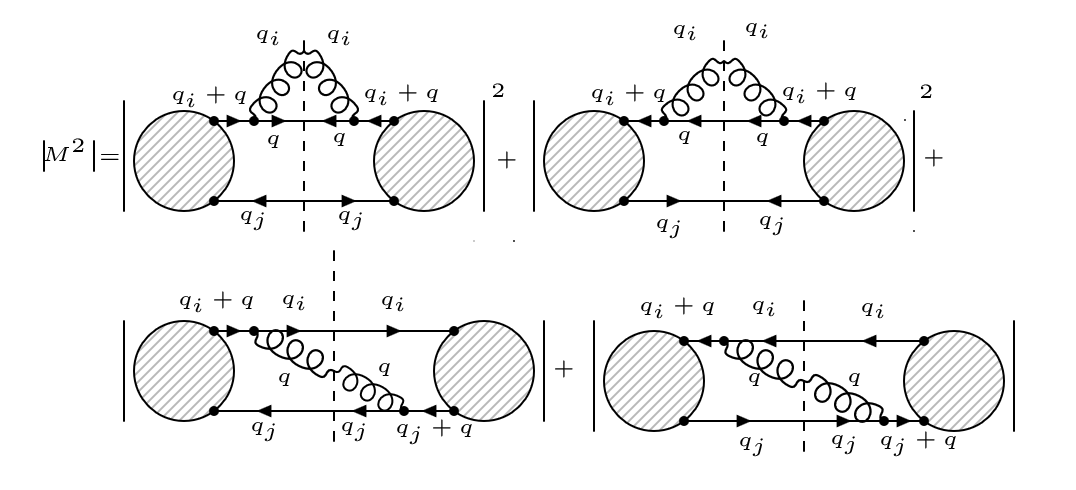
\includegraphics[width=0.85\textwidth]{images/qqgMSquer.png}
\end{figure}
\begin{equation}
\lvert\:M\lvert^2\: = \lvert\:M_1\lvert^2\:+\lvert\:M_2\lvert^2\:+ {\color[RGB]{255,0,0} 2RE(M_1\: {M_2}^{\dagger})}
\end{equation}
\begin{figure}[h!]
\centering
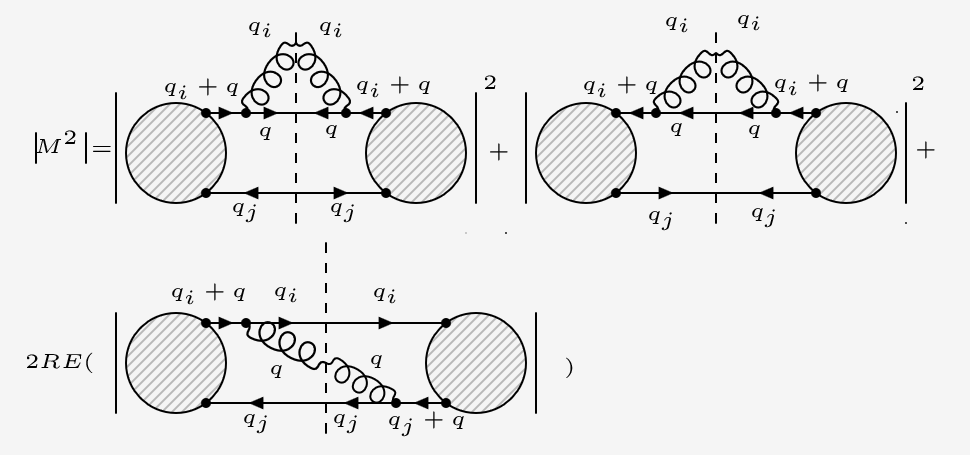
\includegraphics[width=0.85\textwidth]{images/REqqgMSquer.png}
\end{figure}
\begin{equation}
\begin{split}
\lvert\:M\lvert^2\: = (d-2)(1-z)(1-y)\:\frac{g_s^2  {[T^a]_{o}}^k \: {[T^a]_o}^l }{2y(1-2z+2z^2)(p_i \cdot p_j)}
[\not{p_i}][\not{p_j}]\\
-(d-2)yz^2\:\frac{g_s^2 \: {[T^c]_f}^m \: {[T^c]_{f}}^n }{2(1-z)(1-y)(p_i \cdot p_j)}
[\not{p_i}][\not{p_j}]\\
+2RE((\frac{-2z}{z-1}) \frac{g_s^2 \:\:{[T^a]_o}^l \:{[T^a]_{f}}^n }{2y(1-2z+2z^2)(p_i \cdot p_j)} 
[\not{p_i}][\not{p_j}])
\end{split}
\end{equation}

\begin{equation}
{T^a}_{o\:k} \: {T^a}_{l\:o} = \frac{1}{2}(\delta_{oo}\delta_{lk}-\frac{1}{N}\delta_{ok}\delta_{lo})= \frac{1}{2}(N\delta_{lk}-\frac{1}{N}\delta_{lk})=C_F \delta_{lk}
\end{equation}
After summation over the final colour states and averaging over initial colour states we get:

\begin{equation}
{T^a}_{o\:k} \: {T^a}_{l\:o}=C_F \delta_{lk}=\frac{1}{N} \displaystyle\sum\limits_{l=1}^ N \delta_{lk}C_F=C_F
\end{equation}
The same calculation for $ {T^c}_{m\:f} \: {T^c}_{f\:n} $ and $ {T^a}_{o\:l} \: {T^a}_{f\:n} $ turns $ C_F $ out as the colour factor.
Now we are going to compute the splitting function in the case of the colinearity, wich means, if:
\begin{equation}
y \longrightarrow 0
\end{equation}

\begin{equation}
\begin{split}
\lvert\:M\lvert^2\: = (d-2)(1-z)(1-y)\:\frac{g_s^2 C_F}{2y(1-2z+2z^2)(p_i \cdot p_j)}
[\not{p_i}][\not{p_j}]\\
-(d-2)yz^2\:\frac{g_s^2 \: C_F }{2(1-z)(1-y)(p_i \cdot p_j)}
[\not{p_i}][\not{p_j}]\\
+2RE((\frac{-2z}{z-1}) \frac{g_s^2 C_F}{2y(1-2z+2z^2)(p_i \cdot p_j)} 
[\not{p_i}][\not{p_j}]
\end{split}
\end{equation}

\begin{equation}
\lvert\:M\lvert^2\: = C_F((d-2)(1-z)-\frac{4z}{z-1})\:\frac{g_s^2}{2y(1-2z+2z^2)(p_i \cdot p_j)}[\not{p_i}][\not{p_j}]
\end{equation}
for
\begin{equation}
d=4-2\epsilon
\end{equation}

\begin{equation}
\begin{split}
\lvert\:M\lvert^2\: = C_F((4-2\epsilon-2)(1-z)+\frac{4z}{1-z})\:\frac{g_s^2}{2y(1-2z+2z^2)(p_i \cdot p_j)}[\not{p_i}][\not{p_j}]\\
=C_F(\frac{2(1-\epsilon)(1-z)^2+4z}{1-z})\:\frac{g_s^2}{2y(1-2z+2z^2)(p_i \cdot p_j)}[\not{p_i}][\not{p_j}]\\
C_F(\frac{2-4z+2z^2-\epsilon(1-z)^2+4z}{1-z})\:\frac{g_s^2}{2y(1-2z+2z^2)(p_i \cdot p_j)}[\not{p_i}][\not{p_j}]\\
=C_F(\frac{(1+z^2)}{1-z}-\epsilon(1-z))\:\frac{g_s^2}{y(1-2z+2z^2)(p_i \cdot p_j)}[\not{p_i}][\not{p_j}]\\
=\langle\:\hat{P_{qq}}\rangle\:\frac{g_s^2}{q_i \cdot q}[\not{p_i}][\not{p_j}]\\
\end{split}
\end{equation}

\newpage
